%! TEX root = ../main.tex
% ==============================================================
% IMMUTABLE — generated automatically, do not edit this block
%
% — Provenance ───────────────────────────────────────────────────
%   script            : analysis_scratch/under_and_over_mooring_scatter_k.py
%   computed_in       : analysis_scratch/under_and_over_mooring_scatter_k.py (view: undermooring only (loose300 + loose230), k-axis)
%   plot_type         : damping_undermooring_scatter
%   data_class        : DELEG
%   generated_at      : 2026-05-11T09:34:28
%   findings_doc      : 
%
% — Thesis context ──────────────────────────────────────────────
%   chapter           : 05
%   caption_label     : fig:ch05_damping_undermooring_scatter
%   caption_short     : 
%
% — Filters ────────────────────────────────────────────────────
%   panel             : full
%   wind              : no, full
%   amplitude [V]     : 
%   frequency [Hz]    : 
%   probes            : 
%   run_category      : 
%   quality_flag      : ok
%   mooring           : 
%
% — Data provenance ────────────────────────────────────────────
%   n_runs            : 
%   in_probes_used    : 
%   out_probes_used   : 
%   probe_configs     : 
%   non_final_config_n: 
%   datasets        :
%     PROCESSED-20251005-sixttry6roof-highMooring
%     PROCESSED-20251110-tett6roof-lowMooring
%     PROCESSED-20251110-tett6roof-lowMooring-2
%     PROCESSED-20251112-tett6roof
%     PROCESSED-20251113-tett6roof
%     PROCESSED-20251113-tett6roof-loosepaneltaped
%     PROCESSED-20251113-tett6roof-probeadjusted
%     PROCESSED-20260305-newProbePos-tett6roof
%     PROCESSED-20260306-newProbePos-tett6roof
%     PROCESSED-20260307-ProbPos4_31_FPV_2-tett6roof
%     PROCESSED-20260312-ProbPos4_31_FPV_2-tett6roof
%     PROCESSED-20260313-ProbePos4_31_FPV_2-tett6roof
%     PROCESSED-20260314-ProbePos4_31_FPV_2-tett6roof
%     PROCESSED-20260316-ProbePos4_31_FPV_2-tett6roof
%     PROCESSED-20260316-ProbePos4_31_FPV_2-tett6roof-under9Mooring
%     PROCESSED-20260319-ProbePos4_31_FPV_2-tett6roof-under9Mooring
%     PROCESSED-20260321-ProbePos4_31_FPV_2-tett6roof-under9Mooring-height100-RENAMED
%     PROCESSED-20260323-ProbePos4_31_FPV_2-tett6roof-under9Mooring-height100
%     PROCESSED-20260323-ProbePos4_31_FPV_2-tett6roof-under9Mooring-height136
%     PROCESSED-20260324-ProbePos4_31_FPV_2-tett6roof-under9Mooring-height100
%     PROCESSED-20260325-ProbePos4_31_FPV_2-tett6roof-under9Mooring-height100
%     PROCESSED-20260326-ProbePos4_31_FPV_2-tett6roof-under9Mooring-height100
%     PROCESSED-20260326-ProbePos4_31_FPV_2-tett6roof-under9Mooring-height100-lowrange
%     PROCESSED-20260327-ProbePos4_31_FPV_2-tett6roof-under9Mooring30-height100-lowrange
%   run_paths       :
%     (omitted — aggregate over > threshold runs, see datasets)
%
% — Method / numerical parameters ─────────────────────────────
%   grouper           : 
%   collapse_panels   : 
%   fft_window_hz     : 0.1
%   extra_params      : all PROCESSED-* folders (24). Same filter as the ka sibling ch05_damping_all_data_scatter_ka, restricted to categories: below_loose300_full, below_loose230_full. x-axis = k (rad/m) from dispersion: ω² = gk·tanh(kh), h=0.58 m. Top frequency axis with one tick per used frequency. Thesis-scope band (1.3–1.6 Hz) shaded as a light-blue axvspan. Encoding: same (mooring × panel) scheme as the ka sibling — colour shade encodes mooring (within red/blue families), marker family encodes mooring family (○/□/△ for below; diamond/plus/hex for above_50, hollow on reverse panel). Shared XLIM/YLIM across the two views (under, over).
%
% — Summary stats cited in caption ────────────────────────────
%   stat:n_total      : 214
%   stat:n_below_loose300_full : 70
%   stat:n_below_loose230_full : 144
%   stat:k_min        : 1.8388096400303546
%   stat:k_max        : 13.043204534300154
%   stat:ka_min       : 0.008218167374954868
%   stat:ka_max       : 0.31815277442743956
%   stat:freq_min     : 0.6
%   stat:freq_max     : 1.8
%
% — Subfigures available ───────────────────────────────────────
%     FIGURES/ch05_damping_undermooring_scatter.pdf
% ── end immutable block ─────────────────────────────────────────
\begin{figure}[htbp]
  \centering
  \thispagestyle{empty}
  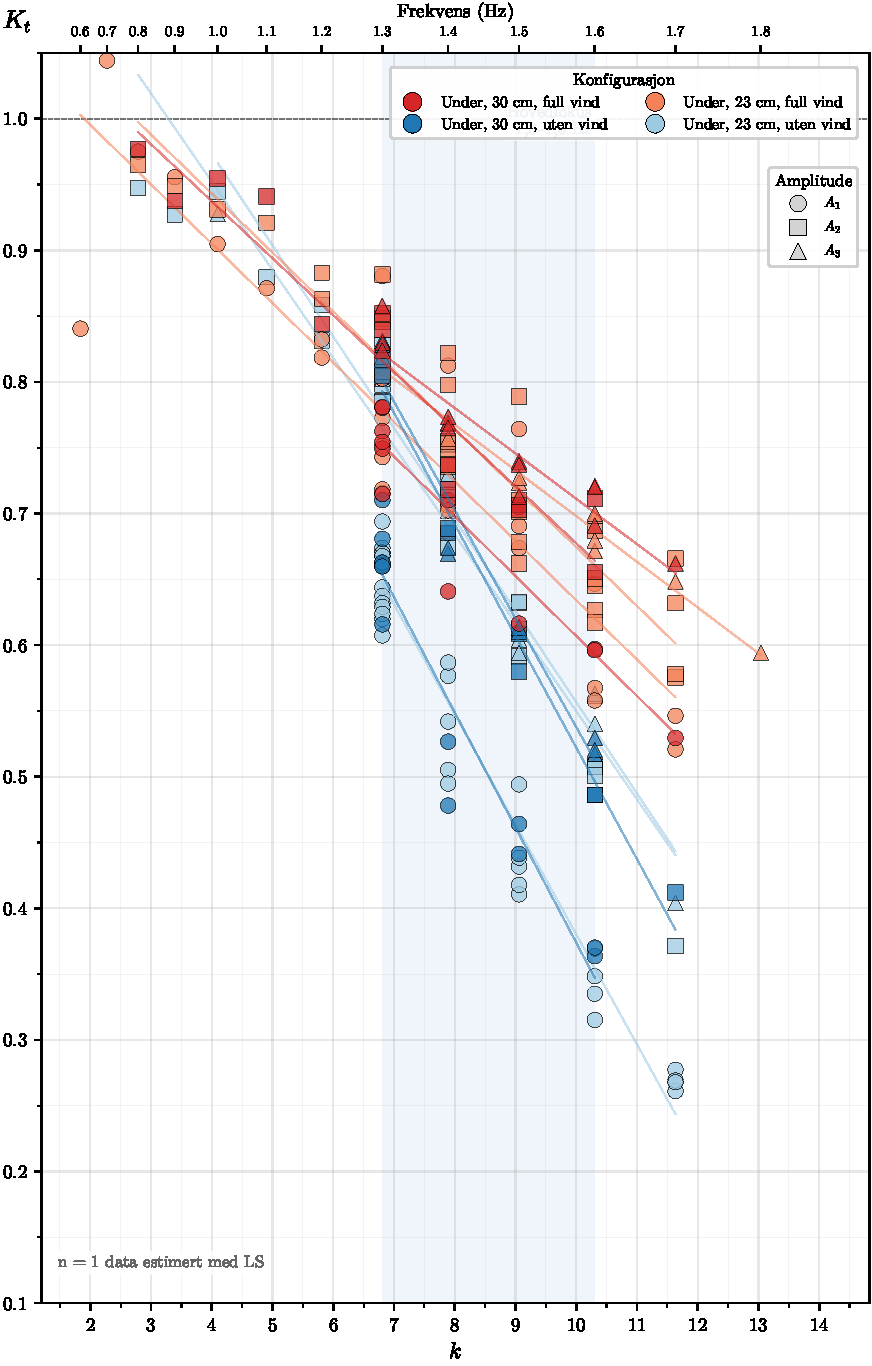
\includegraphics[width=\linewidth]{FIGURES/ch05_damping_undermooring_scatter.pdf}
% >>> CAPTION-SYNC START (do not edit this block; sync_captions.py overwrites)
  \caption{
    % TODO: write caption (edit FIGURE_CAPTIONS/TABLE_CAPTIONS)
  }
% <<< CAPTION-SYNC END
  \label{fig:ch05_damping_undermooring_scatter}
\end{figure}
